\documentclass[11pt,compress]{beamer}
% deactivate beamer navigation
%\setbeamertemplate{navigation symbols}{}
%\usepackage{geometry}
%\geometry{papersize={180mm, 135mm}, top=-1.5mm} % 210mm, 297mm
\usepackage{../style/lmu-lecture}
\setbeamertemplate{frametitle}{\expandafter\uppercase\expandafter\insertframetitle}
%\useoutertheme{metropolis}
% remove section slides
\AtBeginSection[]
{
  \begin{frame}<beamer>
    \frametitle{Introduction to Machine Learning}
    \tableofcontents[currentsection]
  \end{frame}
}
% includepdf slides, pagecommad will set counter for framenumber
\usepackage{pdfpages}
\includepdfset{trim=0mm 0mm 0mm 0mm, pagecommand={\global\setcounter{framenumber}{\value{page}}}}
% trim=0mm 6mm 0mm 0mm, offset=0 15,
% add footer:
\usepackage{framed, color}
\usepackage{xcolor}
%\iffalse
\setbeamertemplate{footline}[text line]{%
    \noindent\hspace*{\dimexpr-\oddsidemargin-1in\relax}%
     \colorbox{white}{
     \makebox[\dimexpr\paperwidth-2\fboxsep\relax]{
     \color{black}
     \begin{minipage}[c][4.5ex][c]{0.5\linewidth}
       \secname
     \end{minipage}
     \hfill\begin{minipage}[c][4.5ex][c]{0.5\linewidth}
       \flushright
       \insertframenumber{}~/~\inserttotalframenumber~~
     \end{minipage}
     }}%
  \hspace*{-\paperwidth}
}
%\fi

\begin{document}
\setbeamercolor{background canvas}{bg=}

% General remark: hyperlinks in included pdfs are not clickable anymore in the combined pdf

\section{Introduction} % 90 min.?
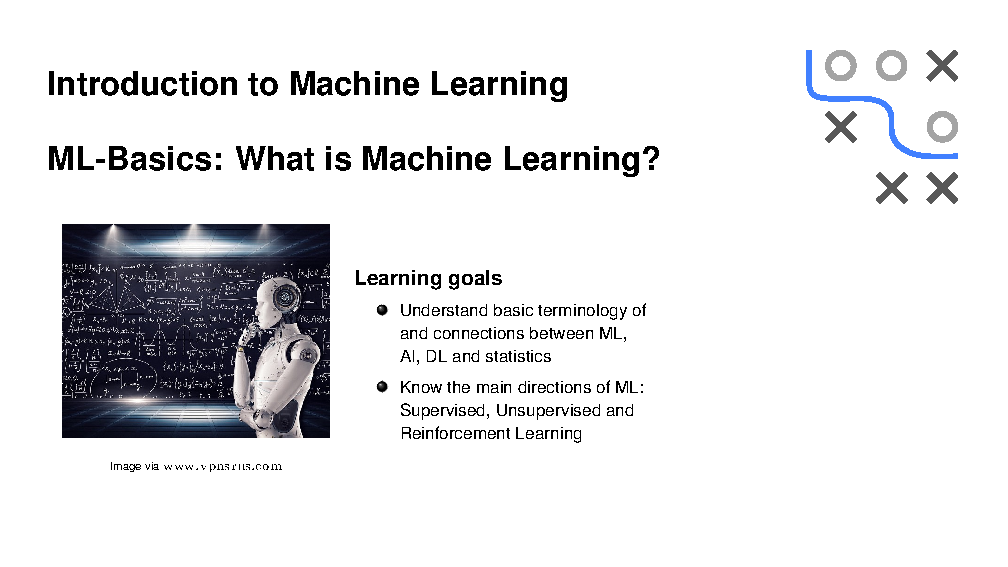
\includepdf[pages={1-7}]{slides-basics-whatisml.pdf}
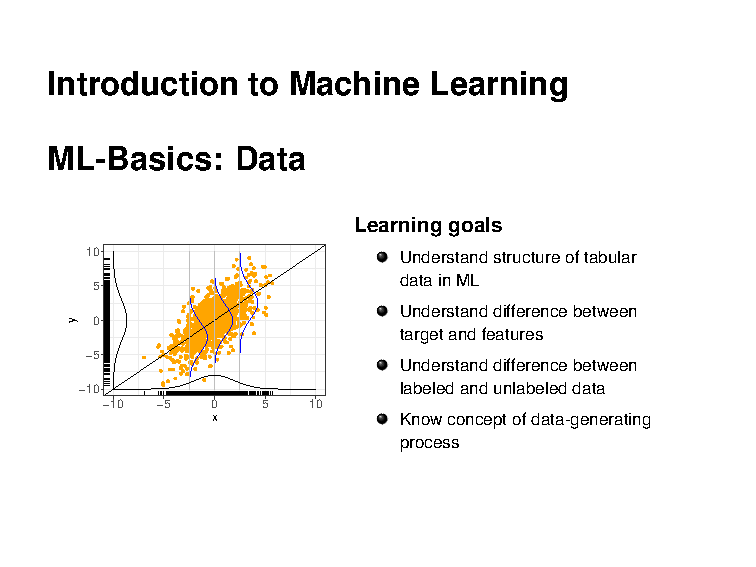
\includepdf[pages={1-6}]{slides-basics-data.pdf}
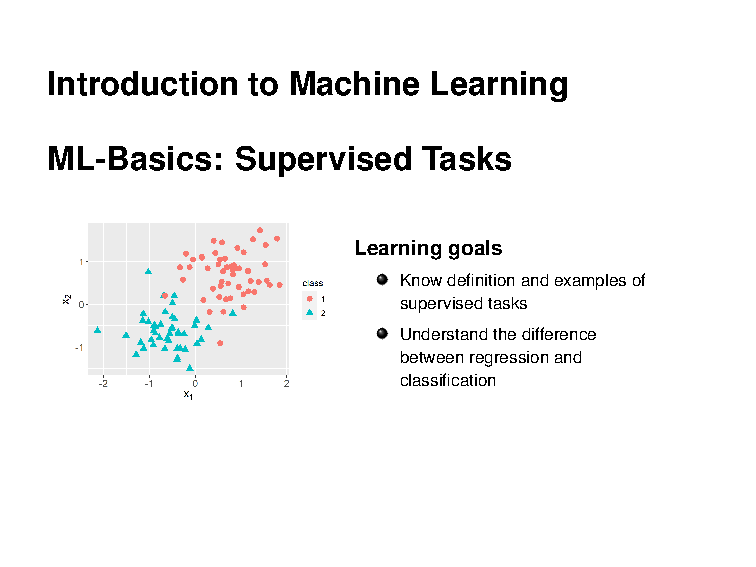
\includepdf[pages={1-last}]{slides-basics-task.pdf}
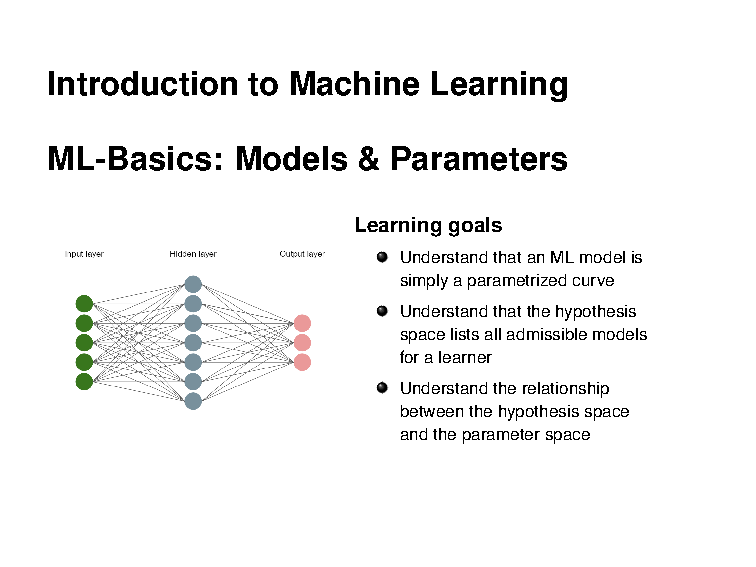
\includepdf[pages={1-8}]{slides-basics-models-parameters.pdf}
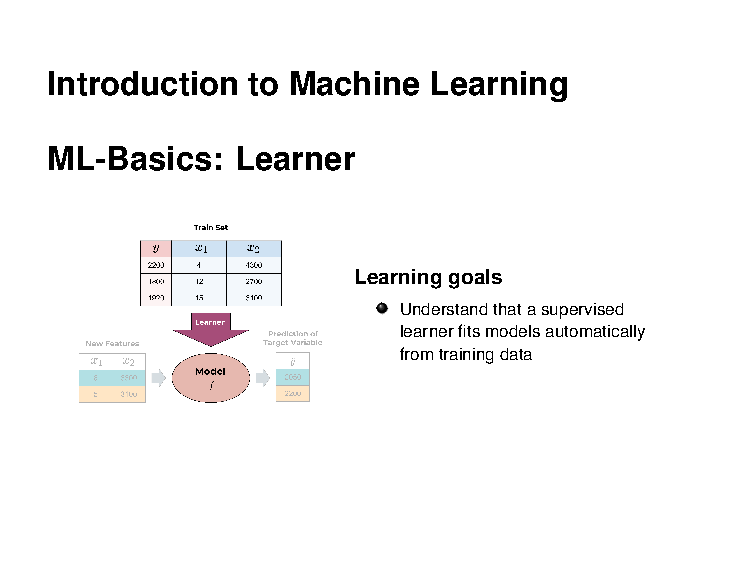
\includepdf[pages={1-last}]{slides-basics-learner.pdf}

\includepdf[pages={1-last}]{slides-basics-riskminimization.pdf}

\section{Performance Measures} % 30 min.?
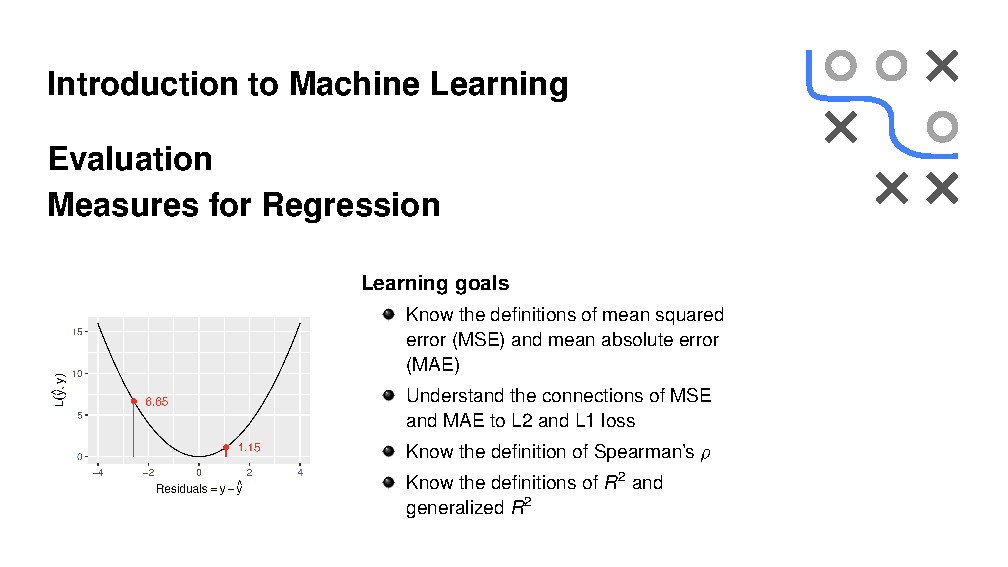
\includepdf[pages={1-3}]{slides-evaluation-measures-regression.pdf}
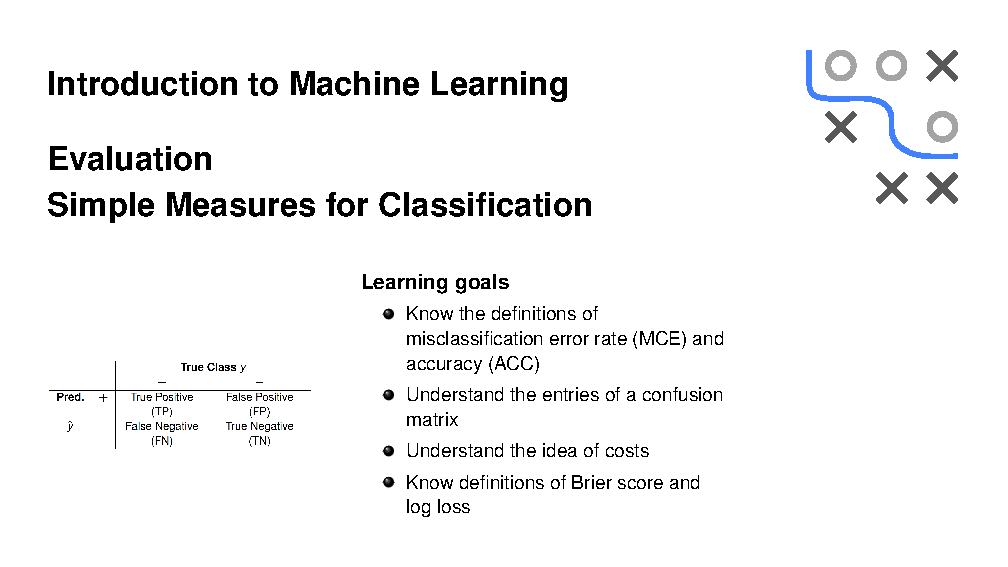
\includepdf[pages={1-5, 8-last}]{slides-evaluation-measures-classification.pdf}
% \section{Supervised Regression}
% %
\includepdf[pages={1-last}]{slides-regression-losses.pdf}
% 
\includepdf[pages={2-12}]{slides-regression-linearmodel.pdf}

\section{Simple ML Algorithms} % 90 min.?
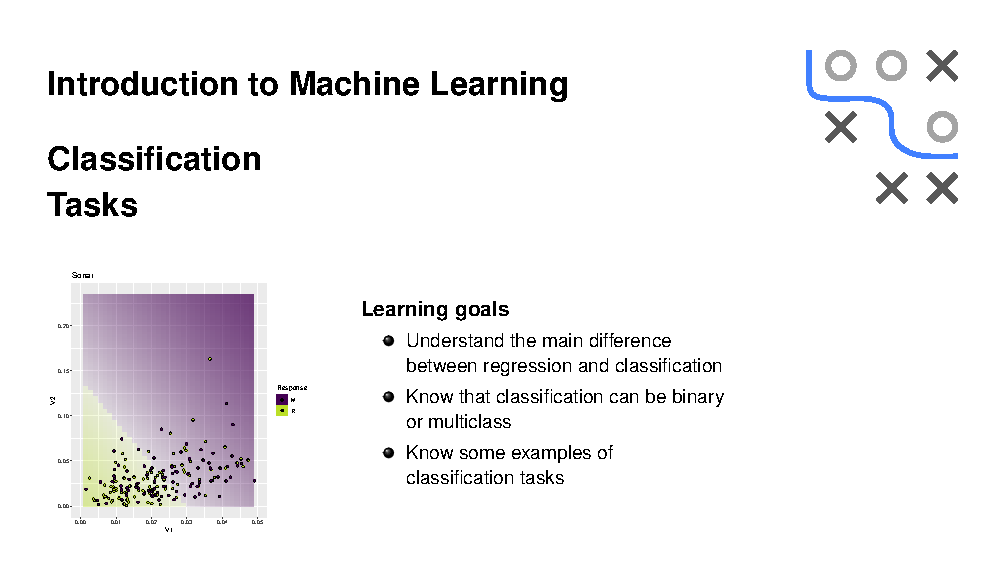
\includepdf[pages={1-last}]{slides-classification-tasks.pdf}
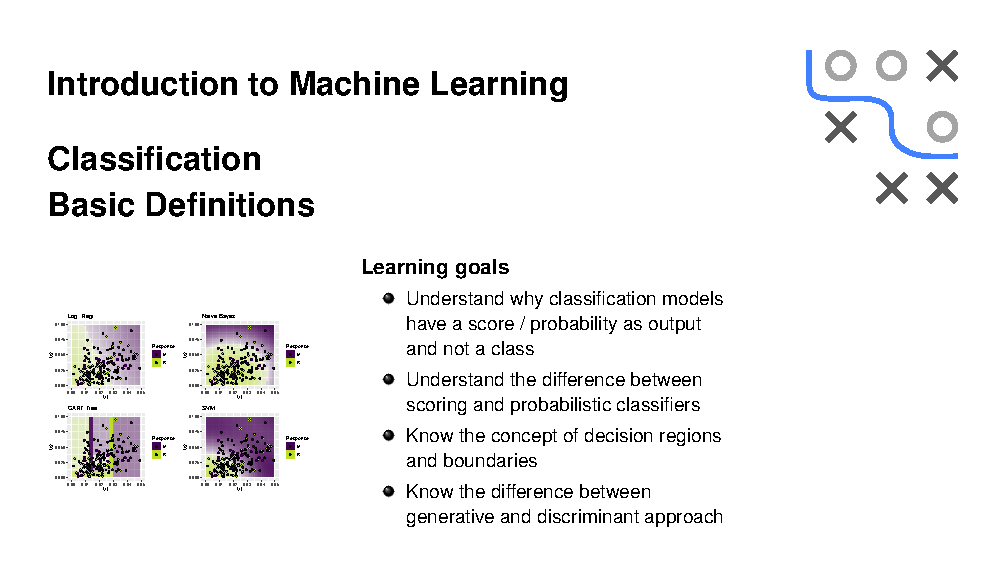
\includepdf[pages={1-9}]{slides-classification-basicdefs.pdf}
%
\includepdf[pages={1-last}]{slides-classification-linear.pdf}
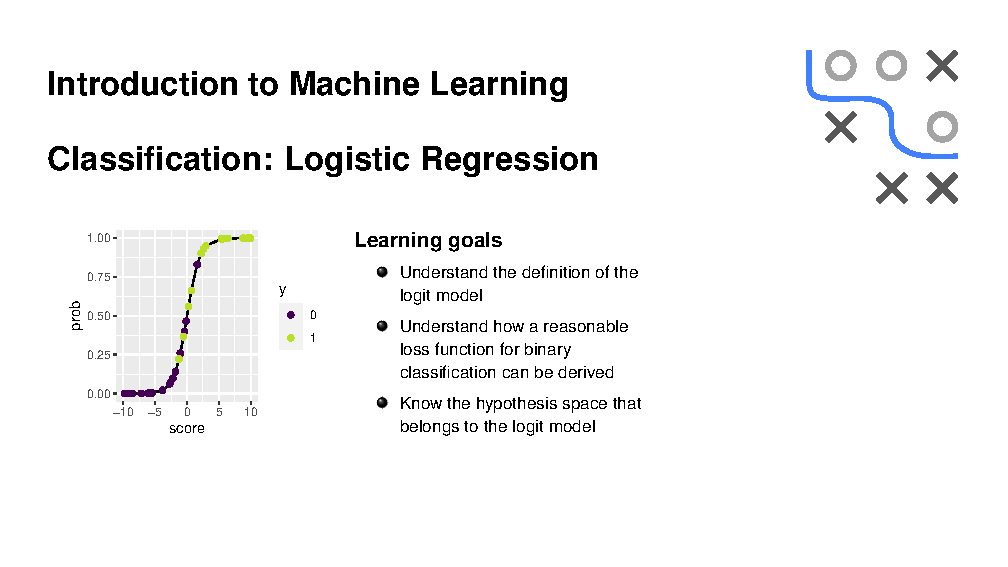
\includepdf[pages={1-last}]{slides-classification-logistic.pdf}
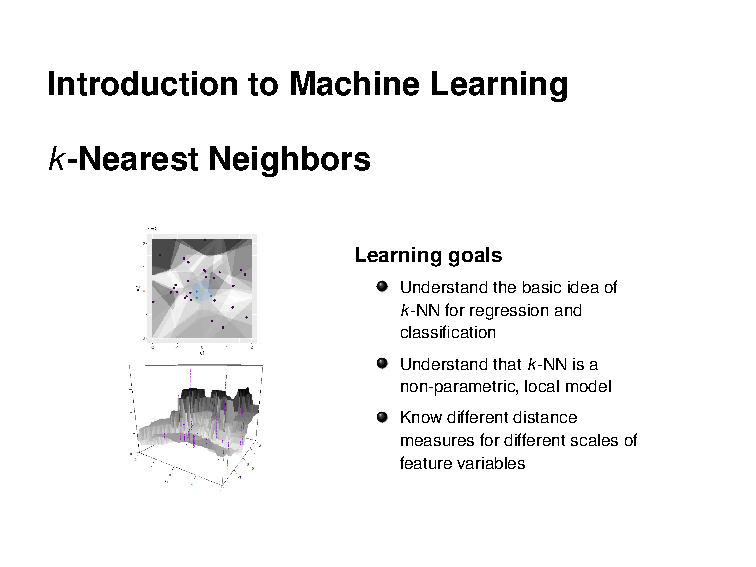
\includepdf[pages={1-7}]{slides-knn.pdf}
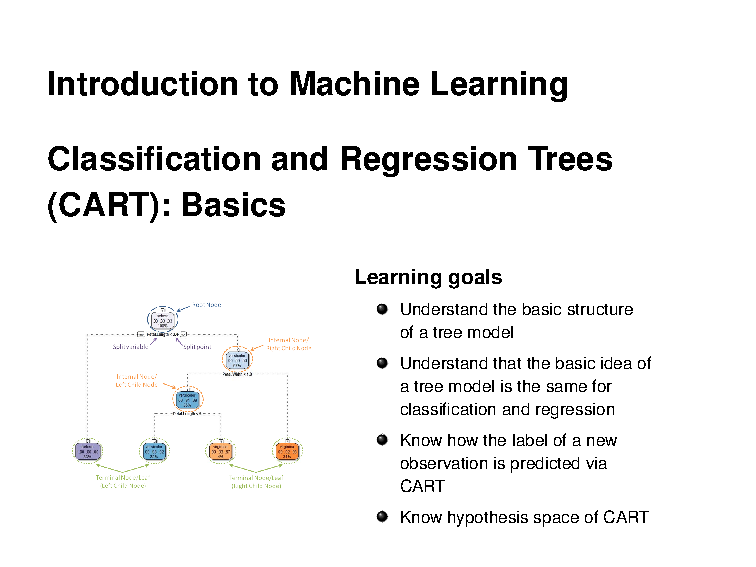
\includepdf[pages={1-last}]{slides-cart-intro.pdf}

\includepdf[pages={1-10}]{slides-cart-splitcriteria.pdf}
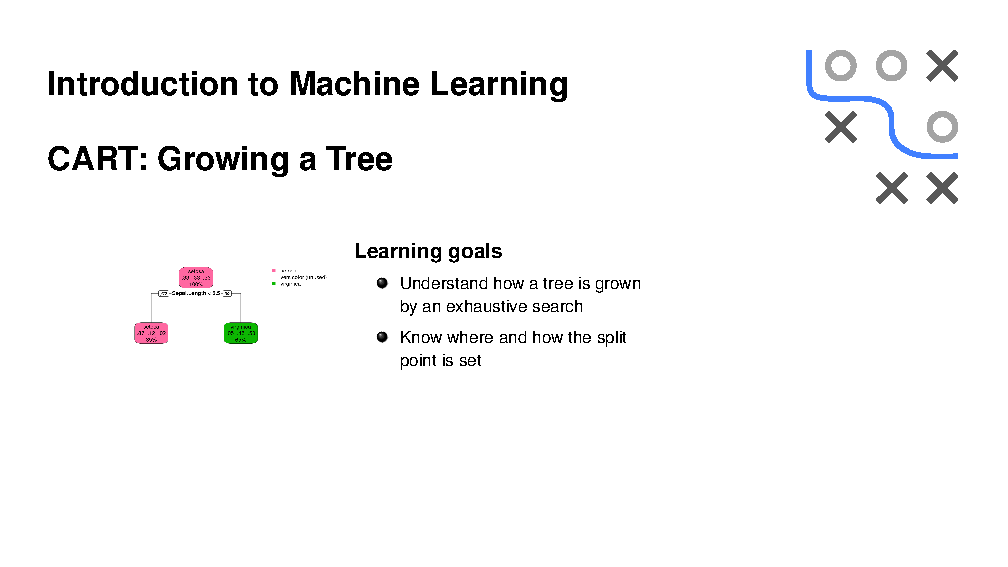
\includepdf[pages={1-last}]{slides-cart-treegrowing.pdf}
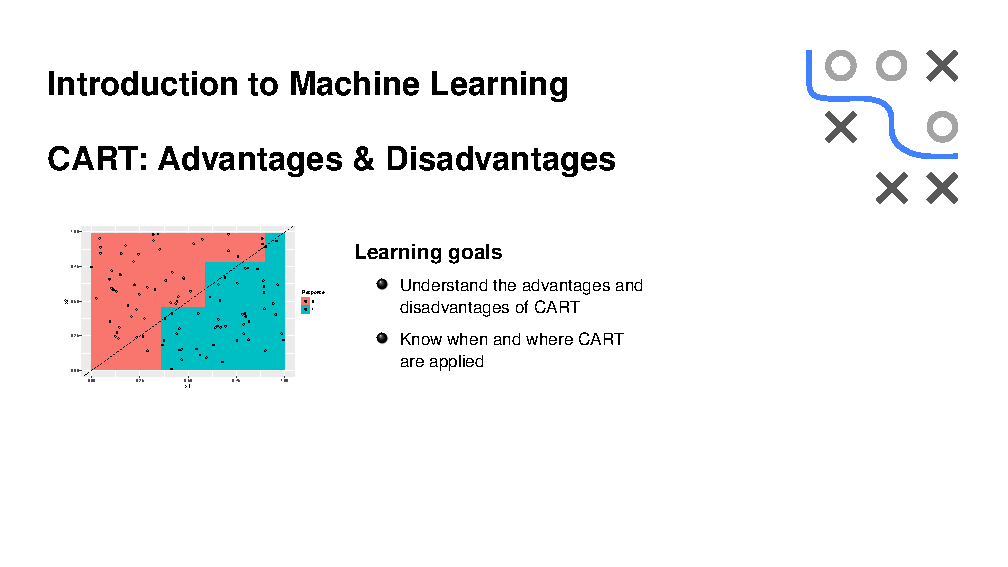
\includepdf[pages={1-7}]{slides-cart-discussion.pdf}

\section{mlr3 Basics} % 60 min. (inkl. use case demo excluding resampling)?

\includepdf[pages={2-last}]{../slides/mlr3/slides-mlr3-intro.pdf}

\section{Exercise: mlr3 Basics} %60 - 90min. (hands-on exercise)?
\begin{frame}{Exercise: mlr3 Basics}
\textbf{Demo:} \href{https://mlr3gallery.mlr-org.com/posts/2020-03-11-basics-german-credit/}{\underline{mlr3 Basics Tutorial}}

\textbf{Exercise:}
\begin{enumerate}
\item Install and load the \texttt{mlr3verse} package and check out the \texttt{iris} data set (see \texttt{?iris} for a description of the data).
\item Train a model on the first \textbf{120 observations} of the \texttt{iris} data set using \texttt{Species} as target feature for prediction. See \texttt{?iris} for the data description and \texttt{as.data.table(mlr\_learners)} for some available learners with their propeties and feature types they can handle (choose a learner you already know which also supports multiclass).
\item Use the trained model to make predictions for the remaining 30 observations (i.e., observations 121-150 from the iris data). What is the classification error on these 30 observations?
% https://mlr3gallery.mlr-org.com/posts/2020-03-18-iris-mlr3-basics/
\end{enumerate}
\end{frame}


\end{document}
